%LaTeX-2e-File, Liedtke, 20140724.
%Inhalt: Einf"uhrung der Ableitung.
%zuletzt bearbeitet: 20140922.

%\begin{MContent}

%%\MSubsubsection{Ableitung--ein Ma"s f"ur die "Anderungsrate der Funktionswerte}
%\MSubsubsection{Zur Idee der Ableitung als ein Ma"s f"ur die "Anderungsrate %
% der Funktionswerte}
\begin{MXContent}{Zur Idee der Ableitung als Ma"s f"ur die "Anderungsrate %
 der Funktionswerte}{Zur Idee der Ableitung}{STD}

Gegeben ist eine Funktion $f: [a, b] \to \R$ und eine Stelle $x_0$ zwischen 
$a$ und $b$.

Wir wollen m"oglichst einfach beschreiben, wie sich die Funktionwerte von 
$f$ lokal, also in der N"ahe einer Stelle $x_0$, "andern.

Eine Gerade beschreibt in einfacher Weise, wie wir von einem Punkt zu einem
anderen kommen k"onnen. Sie kann als vereinfachte, aber weiterhin 
aussagekr"aftige Beschreibung irgendeines {\glqq}krummlinigen{\grqq} Graphen
in einer kleinen Umgebung von einem Punkt angesehen werden.
%In einem ersten Schritt ist eine Gerade $g$ derart gesucht, dass sich die 

Unser Ziel ist es, eine Gerade $g$ derart zu suchen, dass sich die 
Funktionswerte und die "Anderungsraten von $g$ an $f$ \emph{stetig} ann"ahern, 
wenn sich die $x$-Werte an $x_0$ ann"ahern.

Zuerst "uberlegen wir uns, wie wir "Anderungen beschreiben k"onnen. In diesem
Kontext wird dann auch die Idee der stetigen Ann"aherung erl"autert.
%Wir wollen beschreiben, wie sich die Funktionswerte einer Funktion $f$ "andern.
\end{MXContent}

%\MSubsubsection{Absolute und relative "Anderungen}
%\MSubsubsection{Absolute "Anderung}
\begin{MXContent}{Absolute "Anderung}{Absolute "Anderung}{STD}

%Bild:
\begin{center}
\ifttm
\MGraphicsSolo{\MPfadBilder/jb07A1_Funktionsgraph.png}{scale=0.5}
\else
%Datei: {\MPfadBilder/jb07A1_Funktionsgraph.tex}
\begin{small}
\renewcommand{\jTikZScale}{0.7}
\tikzsetnextfilename{jb07A1_Funktionsgraph}
\begin{tikzpicture}[line width=1.5pt,scale=\jTikZScale, %
declare function={
  x0 = 2;
  x1 = 4;
  fkt(\x) = 1/4 * (\x - 1)*(\x - 1) + 0.75;
  rT = 1.6; % relative Translation der Beschriftung $\Delta(f)$
%  Tangente(\x) = 1/2 * (\x - 2) + 1;
}
] %[every node/.style={fill=white}] 
%Koordinatenachsen:
\draw[->] (-0.6, 0) -- ({x1+1}, 0) node[below left]{$x$}; %x-Achse
\draw[->] (0, -0.6) -- (0, {fkt(x1)+1}) node[below left]{$y$}; %y-Achse
%Achsenbeschriftung:
\foreach \x in {1, 2, 3, 4} \draw (\x, 0) -- ++(0, -0.1); %
% node[below] {$\x$}; 
\foreach \y in {1, 2, 3} \draw (0, \y) -- ++(-0.1, 0); %
% node[left] {$\y$};
%\node[below left] at (0, 0) {$0$};
%Hilfslinien:
\draw[color=black!50!white,style=dashed] (x1, {fkt(x0)}) -- (x1, {fkt(x1)});
\draw[color=black!50!white,style=dotted] (x0, {fkt(x0)}) -- (x1, {fkt(x0)});
%Funktion:
\draw[domain=0.5:x1,samples=120,color=\jccolorfkt] %
 plot (\x, {fkt(\x)});
%Punkte und Hilfslinien:
\filldraw[color=black,fill=black] (x0, 0) circle (1pt);
\node[below] at (x0, -0.1) {$x_0$};
\filldraw[color=black,fill=black] (x0, {fkt(x0)}) circle (1pt);
%
\filldraw[color=black,fill=black] (x1, 0) circle (1pt);
\node[below] at (x1, -0.1) {$x$};
%
\filldraw[color=black,fill=black] (x1, {fkt(x0)}) circle (1pt);
\filldraw[color=black,fill=black] (x1, {fkt(x1)}) circle (1pt);
%Beschriftung:
\draw[line width=0.8pt, rounded corners=4pt] %
 ({x1 + rT + 0.0}, 1.0) -- ({x1 + rT + 0.2}, 1.0) -- ({x1 + rT + 0.2}, 2.0) %
 -- ({x1 + rT + 0.4}, 2.0);
\draw[line width=0.8pt, rounded corners=4pt] %
 ({x1 + rT + 0.4}, 2.0) %
 -- ({x1 + rT + 0.2}, 2.0) -- ({x1 + rT + 0.2}, 3.0) -- ({x1 + rT + 0.0}, 3.0);
%
\node[right] at ({x1+rT+0.5}, 2) {$\Delta(f) = f(x) - f(x_0)$};
%
\node[left] at (-0.5, {fkt(x0)}) {$f(x_0)$};
\node[left] at (-0.5, {fkt(x1)}) {$f(x)$};
\end{tikzpicture}
\end{small}
\fi
\end{center}
%Bildende.

Die "Anderung der Funktionswerte zwischen $x$ und $x_0$ ist 
\[
\Delta(f) := f(x) - f(x_0).
\]
Die Differenz $\Delta(f)$ wird auch 
\MEntry{absolute "Anderung}{absolute \"Anderung} von $f$ genannt.
Die Differenz $\Delta(f)$ gibt den Unterschied zwischen $f(x)$ und $f(x_0)$ an.

Viele Funktionen $f$ haben die Eigenschaft, dass die Differenz $\Delta(f)$ 
jedenfalls dann nahezu null ist, wenn nur $x$ nahe genug bei $x_0$ liegt, 
das hei"st, wenn $x - x_0$ nahezu null ist.

Funktionen mit dieser Eigenschaft hei"sen ("uberall) 
\MEntry{stetig}{stetig}, wenn dies f"ur jede Stelle des Definitionsbereichs 
gilt.
%\begin{MExample}
%Beispielsweise gilt dies f"ur $g(x) := 2 x - 1$. Wenn als Abweichung maximal 
%$r := 0,1$ akzeptiert wird, ist f"ur $x_0 := 1$ und alle $x$ mit 
%$1 - \frac{r}{2} < x < 1 + \frac{r}{2}$ dann tats"achlich
%$-0,1 < \Delta(g) < 0,1$.
%\end{MExample}

%Wenn wie hier im Beispiel f"ur beliebig kleine Werte $r > 0$ die Differenz 
%%$\Delta(f)$ immer dann zwischen $-r$ und $r$ liegt -- ihr Betrag also kleiner 
%als $r$ ist, wenn nur $x$ nahe genug bei $x_0$ liegt, dann wird die Funktion 
%$f$ an der Stelle $x_0$ stetig genannt. Und wenn dies f"ur alle Stellen $x_0$ 
%stimmt, hei"st $f$ ("uberall) \MEntry{stetig}{stetig}.

%Bild: Stetige Funktionen -- unstetige Funktionen
\begin{center}
\ifttm
\MGraphicsSolo{\MPfadBilder/jb07A1_DefStetigkeit.png}{scale=0.5}
\else
%Datei: {\MPfadBilder/jb07A1_DefStetigkeit.tex}
\begin{small}
\renewcommand{\jTikZScale}{0.6}
\tikzsetnextfilename{jb07A1_DefStetigkeit}
\begin{tikzpicture}[line width=1.5pt,scale=\jTikZScale]
\begin{scope}[xshift=-9cm]
%\input{\MPfadBilder/jb07A1_DefStetigkeitFolgeLinks.tex}
%LaTeX-File, Liedtke, 20111203.
%MINT-Modul Stetigkeit und Ableitung: Bild Folgenstetigkeit (Folge von links).
%Bildname: jb07A1_DefStetigkeitFolgeLinks.
%Quelle: 20121004, Liedtke.
%bearbeitet: 20140916.

%\tikzsetnextfilename{jb07A1_DefStetigkeitFolgeLinks}
%\begin{small}
%\begin{tikzpicture}[line width=1.5pt,scale=\jTikZScale] % [scale=0.8] 
%[line width=1.5pt, every node/.style={fill=white}] 
%\clip(-1.4,-0.7) rectangle (6.7, 5.7);
%\begin{scope}[xshift=-8cm]
%Koordinatenachsen:
\draw[->] (-0.3, 0) -- (6.6, 0) node[below left]{$x$}; %x-Achse
\draw[->] (0, -0.3) -- (0, 5.6) node[below left]{$y$}; %y-Achse
%Achsenbeschriftung:
%\foreach \x in {1, 2, 3, 4, 5, 6} \draw (\x, 0) -- ++(0, -0.1)%
\foreach \x in {1} \draw (\x, 0) -- ++(0, -0.1)%
 node[below] {$\x$}; 
%\foreach \y in {1, 2, 3, 4} \draw (0, \y) -- ++(-0.1, 0) node[left] {$\y$};
\foreach \y in {1} \draw (0, \y) -- ++(-0.1, 0); % node[left] {$\y$};
\node[below left] at (0, 0) {$0$};
%Funktionsgraph:
%\draw[domain=0:4,color=green!50!black] plot (\x + 1, {1/4*(\x^2) + 1}); 
%\draw[domain=0:5,color=green!50!black] plot (\x + 1/2, {-2*cos(\x/2 r) + 3}); 
\draw[domain=0.8:5.2,samples=200,color=\jccolorfkt] %
 plot (\x, {9/4*sin(3*(\x - 3)/4 r) + 2.7}); 
%Punkte $x$-Achse:
\draw[color=black] (3, 0) circle[radius=1pt];
\foreach \x in {-2, -1, -0.5, -0.25, -0.125} \draw[color=blue] %
 (3 + \x, 0) circle[radius=1pt,fill=blue];
%Punkte Funktionsgraph:
\draw[color=black] (3, 2.7) circle[radius=1pt];
\foreach \x in {-2, -1, -0.5, -0.25, -0.125} \draw[color=blue] %
% (3 + \x, {9/4*sin(3*(3 -\x - 3)/4 r) + 2.7}) circle[radius=1pt]; 
 (3 + \x, {9/4*sin(3*(\x)/4 r) + 2.7}) circle[radius=1pt]; 
%Punkt $y$-Achse:
\draw[color=black] (0, 2.7) circle[radius=1pt];
\foreach \x in {-2, -1, -0.5, -0.25, -0.125} \draw[color=blue] %
 (0, {9/4*sin(3*(\x)/4 r) + 2.7}) circle[radius=1pt,fill=blue];
%Beschriftung:
\node[below] at (2, -0.1) {$x_n$};
\node[below] at (2.5, -0.1) {$\rightarrow$};
\node[below] at (3, -0.1) {$x_0$};
%
\node[left] at (-0.1, {9/4*sin(3*(-1)/4 r) + 2.7}) {$f(x_n)$};
\node[left] at ({-0.1 - 0.25}, {9/4*sin(3*(-0.5)/4 r) + 2.7}) {$\uparrow$};
\node[left] at (-0.1, 2.7) {$f(x_0)$};
%\end{scope}
%\end{tikzpicture}
%\end{small}

%end of file
\end{scope}
\begin{scope}[xshift=0cm]
%\input{\MPfadBilder/jb07A1_DefStetigkeitFolgeRechts.tex}
%LaTeX-File, Liedtke, 20111203.
%MINT-Modul Stetigkeit und Ableitung: Bild Folgenstetigkeit (Folge von rechts).
%Bildname: jb07A1_DefStetigkeitFolgeRechts.
%Quelle 20121004: Liedtke.
%bearbeitet: 20140916, Liedtke.

%\tikzsetnextfilename{jb07A1_DefStetigkeitFolgeRechts}
%\begin{small}
%\begin{tikzpicture}[line width=1.5pt,scale=\jTikZScale] % [scale=0.8] 
%[line width=1.5pt, every node/.style={fill=white}] 
%\clip(-1.4,-0.7) rectangle (6.7, 5.7);
%Koordinatenachsen:
\draw[->] (-0.3, 0) -- (6.6, 0) node[below left]{$x$}; %x-Achse
\draw[->] (0, -0.3) -- (0, 5.6) node[below left]{$y$}; %y-Achse
%Achsenbeschriftung:
%\foreach \x in {1, 2, 3, 4, 5, 6} \draw (\x, 0) -- ++(0, -0.1)%
\foreach \x in {1} \draw (\x, 0) -- ++(0, -0.1)%
 node[below] {$\x$}; 
%\foreach \y in {1, 2, 3, 4} \draw (0, \y) -- ++(-0.1, 0) node[left] {$\y$};
\foreach \y in {1} \draw (0, \y) -- ++(-0.1, 0) node[below left] {$\y$};
\node[below left] at (0, 0) {$0$};
%Funktionsgraph:
%\draw[domain=0:4,color=green!50!black] plot (\x + 1, {1/4*(\x^2) + 1}); 
%\draw[domain=0:5,color=green!50!black] plot (\x + 1/2, {-2*cos(\x/2 r) + 3}); 
\draw[domain=0.8:5.2,samples=200,color=green!50!black] %
 plot (\x, {9/4*sin(3*(\x - 3)/4 r) + 2.7}); 
%Punkte $x$-Achse:
\draw[color=black] (3, 0) circle[radius=1pt];
\foreach \x in {2, 1, 0.5, 0.25, 0.125} \draw[color=blue] %
 (3 + \x, 0) circle[radius=1pt,fill=blue];
%Punkte Funktionsgraph:
\draw[color=black] (3, 2.7) circle[radius=1pt];
\foreach \x in {2, 1, 0.5, 0.25, 0.125} \draw[color=blue]%  
% (3 + \x, {9/4*sin(3*(3 \x - 3)/4 r) + 2.7}) circle[radius=1pt]; 
 (3 + \x, {9/4*sin(3*(\x)/4 r) + 2.7}) circle[radius=1pt]; 
%Punkt $y$-Achse:
\draw[color=black] (0, 2.7) circle[radius=1pt];
\foreach \x in {2, 1, 0.5, 0.25, 0.125} \draw[color=blue] 
 (0, {9/4*sin(3*(\x)/4 r) + 2.7}) circle[radius=1pt,fill=blue];
%Beschriftung:
\node[below] at ({4 + 0.2}, -0.1) {$x_n$};
\node[below] at (3.5, -0.1) {$\leftarrow$};
\node[below] at (3, -0.1) {$x_0$};
%
\node[left] at (-0.1, {9/4*sin(3*(1)/4 r) + 2.7}) {$f(x_n)$};
\node[left] at ({-0.1 - 0.25}, {9/4*sin(3*(0.5)/4 r) + 2.7}) {$\downarrow$};
\node[left] at (-0.1, 2.7) {$f(x_0)$};
%\end{tikzpicture}
%\end{small}

%end of file
\end{scope}
%
\begin{scope}[xshift=9cm]
%\input{\MPfadBilder/jb07A1_BspUnstetigeFktRechts.tex}
%LaTeX-File, Liedtke, 20111203.
%MINT-Modul Stetigkeit und Ableitung: Bild Folgenstetigkeit (Folge von rechts).
%Bildname: jb07A1_BspUnstetigeFktRechts.
%changed 20121004: TikZ-Skalierung via Variable eingef"uhrt.

%\tikzsetnextfilename{jb07A1_BspUnstetigeFktRechts}
%\begin{small}
%\begin{tikzpicture}[line width=1.5pt,scale=\jTikZScale] % [scale=0.8] 
%[line width=1.5pt, every node/.style={fill=white}] 
%\clip(-1.4,-0.7) rectangle (6.7, 5.7);
%Koordinatenachsen:
\draw[->] (-0.3, 0) -- (6.6, 0) node[below left]{$x$}; %x-Achse
\draw[-] (0, -0.3) -- (0, 2.8); %y-Achse
\draw[->] (0, 3.0) -- (0, 5.6) node[below left]{$y$}; %y-Achse
%Achsenbeschriftung:
%\foreach \x in {1, 2, 3, 4, 5, 6} \draw (\x, 0) -- ++(0, -0.1)%
\foreach \x in {1} \draw (\x, 0) -- ++(0, -0.1)%
 node[below] {$\x$}; 
%\foreach \y in {1, 2, 3, 4} \draw (0, \y) -- ++(-0.1, 0) node[left] {$\y$};
\foreach \y in {1} \draw (0, \y) -- ++(-0.1, 0) node[below left] {$\y$};
\node[below left] at (0, 0) {$0$};
%Funktionsgraph:
%\draw[domain=0:4,color=green!50!black] plot (\x + 1, {1/4*(\x^2) + 1}); 
%\draw[domain=0:5,color=green!50!black] plot (\x + 1/2, {-2*cos(\x/2 r) + 3}); 
\draw[domain=0.8:3.0,samples=200,color=green!50!black] %
 plot (\x, {9/4*sin(3*(\x - 3)/4 r) + 2.7}); 
\draw[domain=3.05:5.2,samples=200,color=green!50!black] %
 plot (\x, {9/4*sin(3*(\x - 3)/4 r) + 2.7 + 0.2}); 
%Punkte $x$-Achse:
\draw[color=black] (3, 0) circle[radius=1pt];
\foreach \x in {2, 1, 0.5, 0.25, 0.125} \draw[color=blue] %
 (3 + \x, 0) circle[radius=1pt,fill=blue];
%Punkte Funktionsgraph:
\draw[color=black] (3, 2.7) circle[radius=1pt];
\foreach \x in {2, 1, 0.5, 0.25, 0.125} \draw[color=blue]%  
% (3 + \x, {9/4*sin(3*(3 \x - 3)/4 r) + 2.7}) circle[radius=1pt]; 
 (3 + \x, {9/4*sin(3*(\x)/4 r) + 2.7 + 0.2}) circle[radius=1pt]; 
%Punkt $y$-Achse:
\draw[color=black] (0, 2.7) circle[radius=1pt];
\foreach \x in {2, 1, 0.5, 0.25, 0.125} \draw[color=blue] 
 (0, {9/4*sin(3*(\x)/4 r) + 2.7 + 0.2}) circle[radius=1pt,fill=blue];
%Beschriftung:
\node[below] at ({4 + 0.2}, -0.1) {$x_n$};
\node[below] at (3.5, -0.1) {$\leftarrow$};
\node[below] at (3, -0.1) {$x_0$};
%
\node[left] at (-0.1, {9/4*sin(3*(1)/4 r) + 2.7}) {$f(x_n)$};
\node[left] at ({-0.1 - 0.25}, {9/4*sin(3*(0.5)/4 r) + 2.7}) {$\downarrow$};
\draw[line width=0.5pt,color=red] (-0.82, 3.55) -- (-0.63, 3.65);
\draw[line width=0.8pt,color=red] (-0.3, 2.8) -- (0.3, 3.0);
\node[left] at (-0.1, 2.7) {$f(x_0)$};
%\end{tikzpicture}
%\end{small}

%end of file
\end{scope}
\end{tikzpicture}
\end{small}
\fi
\end{center}
%Bildende.
Das linke und das mittlere Bild zeigen eine stetige Funktion: Je n"aher 
die $x$-Werte bei $x_0$ liegen, desto mehr n"ahern sich die Funktionswerte 
$f(x)$ dem Funktionswert $f(x_0)$ an.
Im rechten Bild ist dies nicht der Fall: Die Funktion ist in $x_0$ nicht 
stetig, kurz unstetig in $x_0$.
\end{MXContent}


%\MSubsubsection{Relative "Anderung}
\begin{MXContent}{Relative "Anderung}{Relative "Anderung}{STD}
In der obigen Betrachtung der absoluten Differenz $\Delta(f)$ der Funktionswerte 
wird noch nicht ber"ucksichtigt, wie weit $x$ von $x_0$ entfernt ist.  
Der Quotient
\[
\frac{\Delta(f)}{\Delta(x)} = \frac{f(x) - f(x_0)}{x - x_0}.
\]
beschreibt, wie sich die Funktionswerte von $f$ im \emph{Vergleich} zum Abstand 
von $x$ zu $x_0$ "andern. 

Der Quotient wird auch \MEntry{relative "Anderung}{relative \"Anderung} genannt
%und wird hier mit \MEntry{diskreter "Anderungsrate}{diskrete \"Anderungsrate} 
und wird hier mit \MEntry{mittlerer "Anderungsrate}{mittlerer \"Anderungsrate} 
bezeichnet. 
Wenn der Grenzwert f"ur $x \to x_0$ exisitert, beschreibt dieser die lokale 
"Anderungsrate:
\[
\lim_{x \to x_0} \frac{\Delta(f)}{\Delta(x)} 
 = \lim_{x \to x_0} \frac{f(x) - f(x_0)}{x - x_0} %%
\] 
Dieser Grenzwert ist somit ein Ma"s daf"ur, wie sich die 
Funktionswerte in der N"ahe von $x_0$ "andern. Er wird Ableitung von $f$ in 
$x_0$ genannt. Wie die Formel mit der urspr"unglichen Idee zusammenh"angt, 
den Verlauf der Funktion n"aherungsweise durch eine Gerade zu beschreiben,
sehen wir uns nun an, nachdem alle wichtigen Begriffe vorgestellt wurden.
\end{MXContent}


%\MSubsubsection{Ableitung}
\begin{MXContent}{Ableitung}{Ableitung}{STD}

Gesucht ist eine Gerade $g(x) = m \cdot (x - x_0) + b$, die sich $f$ in $x_0$ 
stetig ann"ahert, und zwar
\begin{itemize}
\item sowohl mit Blick auf die Funktionswerte
\item als auch mit Blick auf die "Anderungsraten.
\end{itemize}

Somit soll $f(x) - g(x)$ in $x_0$ stetig gegen null streben, also
$0 = f(x_0) - g(x_0)$ und damit $b = g(x_0) = f(x_0)$ sein.

Zudem soll die Restfunktion
\[
r(x) := \frac{\Delta(f)}{\Delta(x)} - \frac{\Delta(g)}{\Delta(x)} %%
 = \frac{f(x) - f(x_0)}{x - x_0} - \frac{g(x) - g(x_0)}{x - x_0} %%
\]
stetig gegen null streben, wenn $x \to x_0$ strebt.

Mit $g(x) = f(x_0) + m (x - x_0)$ und damit $g(x_0) = f(x_0)$ ist
\begin{eqnarray*}
r(x) & = & \frac{\Delta(f)}{\Delta(x)} - \frac{\Delta(g)}{\Delta(x)} \\
 & = & \frac{f(x) - f(x_0)}{x - x_0} - \frac{g(x) - g(x_0)}{x - x_0} \\
 & = & \frac{f(x) - f(x_0) - m \cdot (x - x_0)}{x - x_0} \\
\end{eqnarray*}
Multiplikation mit $x - x_0$ f"uhrt auf
$(x - x_0) r(x) = f(x) - f(x_0) - m \cdot (x - x_0)$, 
woraus dann %%% f"ur $f(x)$ dann
\begin{eqnarray*}
f(x) & = & f(x_0) + m \cdot (x - x_0) + r(x) \cdot (x - x_0) %%
\end{eqnarray*}
folgt.

\begin{MXInfo}{Ableitung}
Wenn es eine in $x_0$ stetige Funktion $r$ mit $r(x_0) = 0$ und eine Gerade 
$g$ mit $g(x) = f(x_0) + m (x - x_0)$ derart gibt, dass die Funktion
%die Funktionswerte $f(x)$ f"ur alle $x$ aus dem Definitionsbereich von $f$ 
in der Form
\[
f(x) = g(x) + r(x) \cdot (x - x_0)
\]
%\[
%f(x) = f(x_0) + m \cdot (x - x_0) + r(x) \cdot (x - x_0)
%\]
%f"ur alle $x$ aus dem Definitionsbereich von $f$ gilt,
geschrieben werden kann,
dann hei"st $f$ in $x_0$ \MEntry{differenzierbar}{differenzierbar}. 
Der eindeutige Wert $m$ wird die \MEntry{Ableitung}{Ableitung} 
von $f$ in $x_0$ genannt.
\end{MXInfo}

%Bild:
\begin{center}
\ifttm
\MGraphicsSolo{\MPfadBilder/jb07A1_Ableitung.png}{scale=0.5}
\else
\begin{small}
\renewcommand{\jTikZScale}{1.0}
%Datei: {\MPfadBilder/jb07A1_Ableitung.tex}

%LaTeX-File, Liedtke, 20140825.
%VBKM-Modul 7 Differentialrechnung: Bild zur Definition der Ableitung
%Bildname: jb07A1_Ableitung.tex.
%Erstellt: 20140825, Liedtke.
%Bearbeitet: 20140829, Liedtke.
%Bearbeitet: 20140901, Liedtke (Dateiname ohne Endung erfasst).

\tikzsetnextfilename{jb07A1_Ableitung}
\begin{tikzpicture}[line width=1.5pt,scale=\jTikZScale, %
declare function={
  x0 = 2;
  x1 = 4;
  fkt(\x) = 1/4 * (\x - 1)*(\x - 1) + 0.75;
  Tangente(\x) = 1/2 * (\x - 2) + 1;
}
] %[every node/.style={fill=white}] 
%Koordinatenachsen:
\draw[->] (-0.6, 0) -- ({x1+1}, 0) node[below left]{$x$}; %x-Achse
\draw[->] (0, -0.6) -- (0, {fkt(x1)+1}) node[below left]{$y$}; %y-Achse
%Achsenbeschriftung:
\foreach \x in {1, 2, 3, 4} \draw (\x, 0) -- ++(0, -0.1); %
% node[below] {$\x$}; 
\foreach \y in {1, 2, 3} \draw (0, \y) -- ++(-0.1, 0); %
% node[left] {$\y$};
%\node[below left] at (0, 0) {$0$};
%Hilfslinien:
\draw[color=black!50!white,style=dashed] (x1, 0) -- (x1, {fkt(x1)});
\draw[color=black!50!white,style=dotted] (x0, {fkt(x0)}) -- (x1, {fkt(x0)});
%Funktion:
\draw[domain=0.5:x1,samples=120,color=\jccolorfkt] %
 plot (\x, {fkt(\x)});
%Tangente:
\draw[domain=0.5:x1,samples=120,color=blue!50!white] %
 plot (\x, {Tangente(\x)});
%Punkte und Hilfslinien:
\filldraw[color=black,fill=black] (x0, 0) circle (1pt);
\node[below] at (x0, -0.1) {$x_0$};
\filldraw[color=black,fill=black] (x0, {fkt(x0)}) circle (1pt);
%
\filldraw[color=black,fill=black] (x1, 0) circle (1pt);
\node[below] at (x1, -0.1) {$x$};
%
\filldraw[color=black,fill=black] (x1, {fkt(x0)}) circle (1pt);
\filldraw[color=black,fill=black] (x1, {Tangente(x1)}) circle (1pt);
\filldraw[color=black,fill=black] (x1, {fkt(x1)}) circle (1pt);
%Beschriftung:
\node[right] at ({x1 + 0.5}, 0.5) {$f(x_0)$};
\node[right] at ({x1 + 0.5}, 1.5) {$m\cdot(x-x_0)$};
\node[right] at ({x1 + 0.5}, 2.5) {$r(x)\cdot(x-x_0)$};
%
\draw[line width=0.8pt, rounded corners=3pt] %
 ({x1 + 0.2}, 0.0) -- ({x1 + 0.3}, 0.0) -- ({x1 + 0.3}, 0.5) %
 -- ({x1 + 0.4}, 0.5); %
\draw[line width=0.8pt, rounded corners=3pt] %
 ({x1 + 0.4}, 0.5)  %
 -- ({x1 + 0.3}, 0.5) -- ({x1 + 0.3}, 1.0) -- ({x1 + 0.2}, 1.0);
%
%
\draw[line width=0.8pt, rounded corners=3pt] %
 ({x1 + 0.2}, 1.0) -- ({x1 + 0.3}, 1.0) -- ({x1 + 0.3}, 1.5) %
 -- ({x1 + 0.4}, 1.5); %
\draw[line width=0.8pt, rounded corners=3pt] %
 ({x1 + 0.4}, 1.5)  %
 -- ({x1 + 0.3}, 1.5) -- ({x1 + 0.3}, 2.0) -- ({x1 + 0.2}, 2.0);
%
%
\draw[line width=0.8pt, rounded corners=4pt] %
 ({x1 + 0.2}, 2.0) -- ({x1 + 0.3}, 2.0) -- ({x1 + 0.3}, 2.5) %
 -- ({x1 + 0.4}, 2.5); %
\draw[line width=0.8pt, rounded corners=3pt] %
 ({x1 + 0.4}, 2.5) %
 -- ({x1 + 0.3}, 2.5) -- ({x1 + 0.3}, 3.0) -- ({x1 + 0.2}, 3.0);
%
%
\draw[line width=0.8pt, rounded corners=4pt] %
 ({x1 + 3.0}, 1.0) -- ({x1 + 3.2}, 1.0) -- ({x1 + 3.2}, 2.0) %
 -- ({x1 + 3.4}, 2.0) %
 -- ({x1 + 3.2}, 2.0) -- ({x1 + 3.2}, 3.0) -- ({x1 + 3.0}, 3.0);
%
\node[right] at ({x1+3.5}, 2) {$\Delta(f) = (m+r(x))\cdot(x-x_0)$};
%
\node[left] at (-0.5, {fkt(x0)}) {$f(x_0)$};
\node[left] at (-0.5, {Tangente(x1)}) {$g(x)$};
\node[left] at (-0.5, {fkt(x1)}) {$f(x)$};
\end{tikzpicture}
\end{small}

%end of file
\fi
\end{center}
%Bildende.

Der Wert $m$ ist tats"achlich eindeutig bestimmt, wie folgende "Uberlegung 
verdeutlicht: Da $r$ stetig ist, gilt
$r(x_0) = r\left(\lim_{x \to x_0} x\right) = \lim_{x \to x_0} r(x)$ und damit
\[
0 = r(x_0) = \lim_{x \to x_0} r(x) %
 = \lim_{x \to x_0} \frac{f(x) - f(x_0) - m \cdot (x - x_0)}{x - x_0} %
 =  \lim_{x \to x_0} \left[\frac{f(x) - f(x_0)}{x - x_0} - m\right]. %%
\]
Hieraus folgt, dass $m$ die eindeutige Zahl
$m = \displaystyle\lim_{x \to x_0} \frac{f(x) - f(x_0)}{x - x_0}$ ist.

\begin{MXInfo}{Schreibweisen der Ableitung}
Damit man sich nicht immer so kompliziert ausdr"ucken muss, wird eine kurze
pr"agnante Schreibweise eingef"uhrt:
Der eindeutig bestimmte Wert $m$ wird mit 
\[
\frac{\MD f}{\MD x}(x_0) := m \quad \text{oder noch k"urzer} \quad f'(x_0) := m %%
\]
bezeichnet.

Die erste Notation wird auch nach Leibniz benannt.
\end{MXInfo}

Wenn die Ableitung mittels des 
Differenzenquotienten $\frac{f(x) - f(x_0)}{x - x_0}$ berechnet werden muss,
bietet es sich oft an, den Differenzenquotienten anders aufzuschreiben. Indem
die Differenz von $x$ und $x_0$ mit $h := x - x_0$ bezeichnet wird, 

%Bild:
\begin{center}
\ifttm
\MGraphicsSolo{\MPfadBilder/jb07A1_AbstandReellerZahlen.png}{scale=0.5}
\else
%Datei: {\MPfadBilder/jb07A1_AbstandReellerZahlen.tex}
\begin{small}
\renewcommand{\jTikZScale}{0.7}
\tikzsetnextfilename{jb07A1_AbstandReellerZahlen}
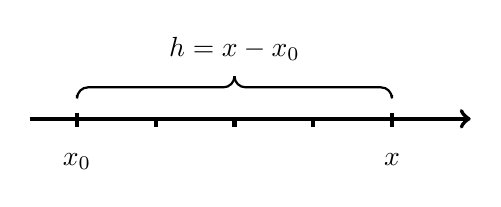
\begin{tikzpicture}[line width=1.5pt,scale=\jTikZScale, %
declare function={
  x0 = 0;
  x1 = 4;
}
] %[every node/.style={fill=white}] 
%Koordinatenachsen:
\draw[->] (-0.6, 0) -- ({x1+1}, 0); % node[below left]{$x$}; %x-Achse
%Achsenbeschriftung:
\foreach \x in {0, 1, 2, 3, 4} \draw (\x, 0.0) -- ++(0, -0.1); %
\foreach \x in {0, 4} \draw (\x, 0.0) -- ++(0, +0.08); %
% node[below] {$\x$}; 
%Beschriftung:
%\draw[line width=0.8pt, rounded corners=4pt] %
% (0, 0.3) -- (0, 0.4) -- (2, 0.4) -- (2, 0.5);
\draw[line width=0.8pt, rounded corners=4pt] %
 ({x0}, 0.3) -- ({x0}, 0.4) -- ({x1/2}, 0.4) %
 -- ({x1/2}, 0.5);
\draw[line width=0.8pt, rounded corners=4pt] %
 ({x1/2}, 0.5)
 -- ({x1/2}, 0.4) -- ({x1}, 0.4) -- ({x1}, 0.3);
%
\node[above] at ({x1/2}, 0.6) {$h = x - x_0$};
%
\node[below] at ({x0}, -0.3) {$x_0$};
\node[below] at ({x1}, -0.3) {$x$};
\end{tikzpicture}
\end{small}
\fi
\end{center}
%Bildende.

ist wegen $x = x_0 + h$ dann
\[
\frac{f(x) - f(x_0)}{x - x_0} = \frac{f(x_0 + h) - f(x_0)}{h}
\]
Hier ist nun der Grenzwert f"ur $h \to 0$ zu betrachten, um die Ableitung zu
berechnen: 
\[
f'(x_0) = \lim_{x \to x_0} \frac{f(x) - f(x_0)}{x - x_0} %
 = \lim_{h \to 0} \frac{f(x_0 + h) - f(x_0)}{h}
\]
Viele der oft benutzten Funktionen sind differenzierbar, wie im Folgenden 
erl"autert wird. 

Die Betragsfunktion $f(x) := |x|$ ist ein einfaches Beispiel 
daf"ur, dass eine stetige Funktion nicht unbedingt differenzierbar zu sein 
braucht. 

\begin{MExample}
Die Betragsfunktion ist an der Stelle $x_0 = 0$ nicht differenzierbar.
Wenn n"amlich f"ur $f$ an der Stelle $x_0 = 0$ der Differenzenquotient
\[
\frac{f(0+h) - f(0)}{h} = \frac{|h|}{h}
\]
f"ur $h < 0$ betrachtet wird, ergibt sich $-1$, und f"ur $h > 0$ ist er 
gleich $1$, sodass der Grenzwert f"ur $h \to 0$ nicht existiert und somit die 
Betragsfunktion an der Stelle $x_0 = 0$ nicht differenzierbar ist.

Der Verlauf des Graphen "andert seine Richtung an der Stelle $(0, 0)$ sprunghaft: 
Salopp
ausgedr"uckt, weist der Funktionsgraph an der Stelle $(0, 0)$ einen Knick auf.
%Bild:
\begin{center}
\ifttm
\MUGraphicsSolo{\MPfadBilder/jb07A1_BspBetragsfunktion.png}{scale=0.5}{}
\else
%Datei: {\MPfadBilder/jb07A1_BspBetragsfunktion.tex}
\renewcommand{\jTikZScale}{1.0}
\tikzsetnextfilename{jb07A1_BspBetragsfunktion}
\begin{tikzpicture}[line width=1.5pt,scale=\jTikZScale]
%LaTeX-File, Liedtke, 20140916.
%VBKM-Modul 7 Differentialrechnung: Bild zur Betragsfunktion
%Bildname: jb07A2_BspBetragsfunktion
%Erstellt: 20140916, Liedtke.

%\begin{small}
%\begin{tikzpicture}[line width=1.5pt,scale=\jTikZScale, %
%declare function={
%  fkt(\x) = sin(\x r);
%}
%] %[every node/.style={fill=white}] 
%Koordinatenachsen:
\draw[->] (-3.6, 0) -- (4, 0) node[below left]{$x$}; %x-Achse
\draw[->] (0, -0.6) -- (0, 4.6) node[below left]{$y$}; %y-Achse
%Achsenbeschriftung:
\foreach \x in {-3, -2, -1, 1, 2, 3} \draw (\x, 0) -- ++(0, -0.1) %
 node[below] {$\x$};
\foreach \y in {1, 2, 3, 4} \draw (0, \y) -- ++(-0.1, 0) node[left] {$\y$};
%\node[below left] at (0, 0) {$0$};
%Funktion:
\draw[domain=-3.2:3.2,samples=120,color=\jccolorfkt] %
 plot (\x, {abs(\x)});
%Tangenten im Nullpunkt, wenn $f$ f"ur $x \leq 0$ bzw. $x \geq 0$ betrachtet 
%wird:
\draw[samples=120,color=blue!50!black] %
 (-0.5, 0.5) -- (0.5, -0.5);
\draw[samples=120,color=blue!50!black] %
 (-0.5, -0.5) -- (0.5, 0.5);
%Punkt: Markierung der Stelle $0$:
\filldraw[color=black,fill=black] (0, 0) circle (1pt);
%end of file
\end{tikzpicture}
\fi
\end{center}
%Bildende.
\end{MExample}

Auch wenn eine Funktion unstetig ist, besonders wenn sie eine Sprungstelle hat,
gibt es keine eindeutige Tangente an den Graphen und somit keine Ableitung.

%Bild:
\ifttm
\MUGraphics{\MPfadBilder/jb07A1_BspUnstetigeFkt.png}{scale=0.5}%
{Funktion mit Sprungstelle in $x_0 = 1$}{}
\else
\begin{center}
%Datei: {\MPfadBilder/jb07A1_BspUnstetigeFkt.tex}
\renewcommand{\jTikZScale}{1.0}
\tikzsetnextfilename{jb07A1_BspUnstetigeFkt}
\begin{tikzpicture}[line width=1.5pt,scale=\jTikZScale]
%LaTeX-File, Liedtke, 20140916.
%VBKM-Modul 7 Differentialrechnung: Bild einer unstetigen Funktion
%Bildname: jb07A2_BspUnstetigeFkt.
%Erstellt: 20140916, Liedtke.
%declare function={
%  fkt(\x) = (\x+1)*(\x+1)/4 + 0.5};
%}
%] %[every node/.style={fill=white}] 
%Koordinatenachsen:
\draw[->] (-3.6, 0) -- (4, 0) node[below left]{$x$}; %x-Achse
\draw[->] (0, -0.6) -- (0, 4.2) node[below left]{$y$}; %y-Achse
%Achsenbeschriftung:
\foreach \x in {-3, -2, -1, 1, 2, 3} \draw (\x, 0) -- ++(0, -0.1) %
 node[below] {$\x$};
\foreach \y in {2, 3} \draw (0, \y) -- ++(-0.1, 0) node[left] {$\y$};
%\node[below left] at (0, 0) {$0$};
%Funktion:
\draw[domain=-2.0:1.0,samples=120,color=\jccolorfkt] %
 plot (\x, {(\x+1)*(\x+1)/4 + 0.5});
\draw[domain=1.05:2.0,samples=120,color=\jccolorfkt] %
 plot (\x, {(\x+1)*(\x+1)/4 + 1.5});
%Tangenten in $x_0 = 1$, wenn die stetige Fortsetzung von $f$ f"ur $x \leq 1$ 
%bzw. $x \geq 1$ betrachtet wird:
\draw[samples=120,color=blue!50!black] %
 (0.5, 1.0) -- (1.5, 2.0);
\draw[samples=120,color=blue!50!black] %
 (0.5, 2.0) -- (1.5, 3.0);
%Punkt: Markierung der Stelle $x_0 = 1$:
\filldraw[color=black,fill=black] (1, 0) circle (1pt);
\end{tikzpicture}
\end{center}
\fi
%Bildende.

\end{MXContent}

%\end{MContent}

%end of file.

